\chapter{Introduction}

``Mental pictures'' and ``visual intuition'' capture how people make sense of abstract concepts and see solutions to hard problems in a visual way. Hadamard described numerous examples of mathematicians doing exactly this in \emph{The Mathematician's Mind}~\cite{Hadamard1997a}, later summarized by Alan Kay~\cite{doingWithImages}:

\begin{quote}
Jacques Hadamard, the famous French mathematician, in the late stages of his life, decided to poll his 99 buddies, who made up together the 100 great mathematicians and physicists on the earth, and he asked them, ``How do you do your thing?'' They were all personal friends of his, so they wrote back depositions. Only a few, out of the hundred, claimed to use mathematical symbology at all. Quite a surprise. All of them said they did it mostly in imagery or figurative terms.
\end{quote}

Learning research suggests that visual representations of knowledge are powerful tools for thought. Visual representations like diagrams enable more robust learning \cite{multimediaLearning} and abstract and flexible problem solving~\cite{Koedinger1990a, pictureAlgebra, DiagramsThousandWords}. Importantly, when people work with visuals, they build better conceptual understanding and more flexible mental models that go beyond memorized procedures~\cite{multipleReps}.

\setlength{\columnsep}{1em}
\setlength{\intextsep}{0em}
\begin{wrapfigure}{r}{.45\textwidth}
\vspace{-10pt}
  \begin{center}
    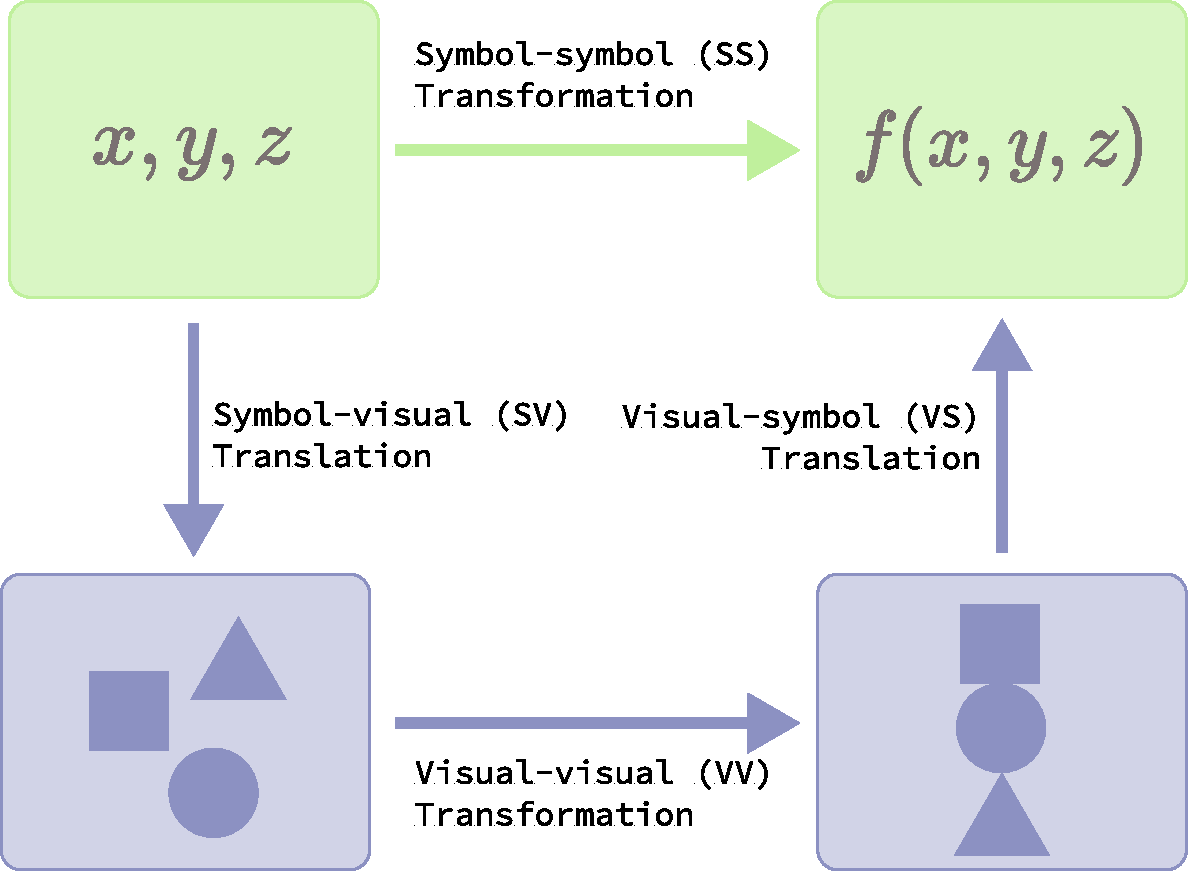
\includegraphics[width=0.45\textwidth]{assets/chapter-1/grounding-rectangle.pdf}
  \end{center}
\end{wrapfigure}

Let me use a diagram to capture this: the \textbf{grounding rectangle} represents two pathways to learning and problem solving: One can perform symbol-to-symbol transformations (SS, or “symbol pushing”) or through an \textcolor[HTML]{8C91C2}{alternative diagrammatic pathway}: a symbol-to-diagram translation (SV), a diagram-to-diagram transformation (VV), and finally a diagram-to-symbol translation (VS).

Research on expertise development suggests a need for substantial exposure involving repetition in varied contexts or deliberate practice \cite{deliberatePractice} to acquire the perceptual chunks \cite{chunkingModels, perceptualLearningExpertise} that support accurate interpretation and use of visual representations~\cite{Koedinger1990a}. Through enough practice, learning the two paths in the grounding rectangle can produce better, more robust memory \cite{dualCoding}, learning~\cite{multipleReps, multimediaLearning, cotraining}, and future reasoning, both in providing flexibility and in supporting error recovery \cite{groundedAndAbstractReps}.

In reality, there seems to be an over-abundance of symbolic practice, continuing Kay's train of thought:

\begin{quote}
    The sad part of the diagram is that every child in the United States is taught math and physics through this [symbolic] channel. The channel that almost no adult creative mathematician or physicist uses to do it... They use this channel to communicate, but not to do their thing.
\end{quote}

Diagrammatic practice is rare due to the significant cost of authoring diagrammatic problems. Existing diagramming tools often require hours of low-level tweaking of geometric primitives and do not capture the core task of diagramming: representing ideas visually. In other words, these tools lack \emph{representational salience}. As a result, the diagrams created by existing tools don't have semantics, as they are merely a collection of pixels and geometric blobs.  

% In prior work, colleagues and I built \Penrose, a diagramming platform that explicitly encodes visual representations in domain-specific languages (DSLs)~\cite{penrose}. In this thesis proposal, I argue that this explicit encoding can be leveraged to (1) reduce the programming effort of producing diagrammatic problems at scale and (2) simplify the workflow of authoring interactive diagrams. The resulting diagrams also carry rich semantics, and I propose to use them to (3) provide useful, automated feedback to students. My thesis statement summarizes the above:

% \vspace{10pt}
% \boxtext{
% \textbf{Encoding visual representations in diagramming tools simplifies programming of interactive visual activities that provide students with automated feedback at scale.}
% }
% \vspace{10pt}

% The expected contributions of this work are:

% \begin{enumerate}
%     \item \emph{Need-finding studies} on challenges authors face.
%     \item \emph{A platform of tools} based on the visual encoding of \Penrose for mass-production of diagrams (\cref{chp:edgeworth}) and rapid authoring of interactive diagrams (\cref{chp:ipenrose}).
%     \item \emph{A theoretical framework} of the grounding rectangle, which guides the design of tools presented in this proposal.
% \end{enumerate}

% \begin{proposed}
% \textbf{Note.} This proposal contains a mix of completed, in-progress, and proposed projects. In the rest of this document, proposed work will be marked in orange on the left margin. 
% \end{proposed}

\section{Research Questions}


%
\subsection{Hypotheses and research questions}

Comparing with related work discussed in \cref{sec:edgeworth-related}, \Edgeworth uniquely support scalable generation of diagrammatic translation problems in multiple domains. Therefore, in this section, I discuss hypotheses that cover the essential features of \Edgeworth such as the mutation-based approach and automatic detection of examples and counterexamples. For each hypothesis, I will also discuss further research questions to be investigated in the evaluation plan. 

\boxtext{\textbf{H1:} Given manageable effort in configuring the mutator, \Edgeworth can reliably generate examples and counterexamples for translation problems with relatively few mutants required.}

An effective translation problem needs to include both examples and counterexamples. Therefore, the technical approach of \Edgeworth---program mutations on \Substance code---must produce them reliably. To verify H1, the following research questions need to be answered:

\begin{itemize}
    \item \textbf{R1.1}: How many mutants does \Edgeworth need to generate to obtain sufficient examples and counterexamples for translation problems?
    \item \textbf{R1.2}: How frequently does \Edgeworth succeed or fail at doing so?
\end{itemize}

The preliminary evaluation showed that the mutator configuration will affect the quality of the mutants. Therefore, I will also address the following research question on mutator configuration and will use the results to further investigate possible ways to lower the configuration burden, e.g. the programming-by-example workflow and changes to the configuration format.

\begin{itemize}
    \item \textbf{R1.3}: How much configuration effort is required to produce examples and counterexamples? 
\end{itemize}

\boxtext{\textbf{H2}: \Edgeworth makes translation problem authoring more efficient.}

The main goal of \Edgeworth is to improve the efficiency of translation problem authoring. To verify H2, the evaluation plan will answer:
\begin{itemize}
    \item  \textbf{R2.1}: Comparing with workflows that authors are using, can \Edgeworth shorten the authoring time of translation problems?
    \item  \textbf{R2.2}: Which aspect(s) of the authoring workflow does \Edgeworth simplify, and does \Edgeworth introduce new authoring difficulties? 
    \item  \textbf{R2.3}: Are authors more efficient using the configuration-based workflow or programming-by-example workflow?
\end{itemize}

Regardless of the answer to R2.1, meaningful results on R2.2 can provide more insights on how \Edgeworth's approach impacts the problem authoring experience. For instance, I postulate that \Edgeworth improves authoring efficiency by (1) simplifying the mechanics of diagram production and (2) reducing the author's effort to come up with examples and counterexamples. On the other hand, \Edgeworth's mutation-based approach may introduce new problems such as difficulties finding the right diagrams from the mutant pool and controlling the quality of examples. The automatic detection heuristics described above aim to mitigate these difficulties.

\boxtext{\textbf{H3}: \Edgeworth can automatically distinguish examples from counterexamples, and this feature helps authors find examples and counterexamples for translation problems.}

The effectiveness of translation problems depends on the choice of examples and counterexamples. I hypothesize that example generation/selection is a nontrivial activity that authors spend time doing, and computational support in \Edgeworth can help authors identify examples/counterexamples. Answering the following research questions will verify H3:

\begin{itemize}
    \item \textbf{R3.1}: Can \Edgeworth automatically detect examples, counterexamples, and edge cases with a reasonably high accuracy?
    \item \textbf{R3.2}: Do the detection results help authors identify potential answers to translation problems?
\end{itemize} \subsection{Limitations}


All the work presented in this proposal was carried out in collaboration with others, and to recognize this, I use ``we'' rather than the singular first person in the subsequent chapters.
